\documentclass{beamer}
%\documentclass[handout]{beamer}

%\setbeamertemplate{background canvas}[vertical shading][bottom=white,top=structure.fg!25]
% or whatever

\usetheme[compress]{Amsterdam}
%\setbeamertemplate{headline}{}
%\setbeamertemplate{footline}{}
%\setbeamersize{text margin left=0.5cm}
  
\usepackage[english]{babel}
\usepackage{listings}
\usepackage{geometry}
\usepackage{hyperref}


\usepackage[utf8]{inputenc}
\usepackage[T1]{fontenc}
\usepackage{lmodern}

\lstset{
basicstyle=\scriptsize\ttfamily,
columns=flexible,
breaklines=true,
numbers=left,
%stepsize=1,
numberstyle=\tiny,
backgroundcolor=\color[rgb]{0.85,0.90,1}
}


\begin{document}

\title[Big Data and Automated Content Analysis]{\textbf{Big Data and Automated Content Analysis} \\ Week 1 -- Wednesday \\ »First steps in the VM«}
\author[Damian Trilling]{Damian Trilling \\ ~ \\ \footnotesize{d.c.trilling@uva.nl \\@damian0604} \\ \url{www.damiantrilling.net}}
\date{7 February 2018}
\institute[UvA]{Afdeling Communicatiewetenschap \\Universiteit van Amsterdam}


\begin{frame}{}
\titlepage
\end{frame}

\begin{frame}{Today}
\tableofcontents
\end{frame}



\section{The Linux command line}

\begin{frame}
	When point-and-click doesn't help you further:\\
	\textbf{The Linux command line}
\end{frame}

\begin{frame}{The tools}
\begin{block}{General idea}
Whereever possbile, we use tools that are
\begin{itemize}
\item platform-independent 
\item free (as in beer and as in speech)
\item open source
\end{itemize}
\end{block}

\onslide<2->{To make things easier, we work with a virtual machine in which everyone runs \emph{the same} Linux version}.

\end{frame}




{\setbeamercolor{background canvas}{bg=black}
	\begin{frame}[plain]
		\makebox[\linewidth]{
			
\includegraphics[width=\paperwidth,height=.9\paperheight,keepaspectratio]{../../pictures/keep-calm-and-start-your-engines.png}
		}
	\end{frame}
}

\begin{frame}{Let's switch to Linux!}
	\makebox[\linewidth]{
		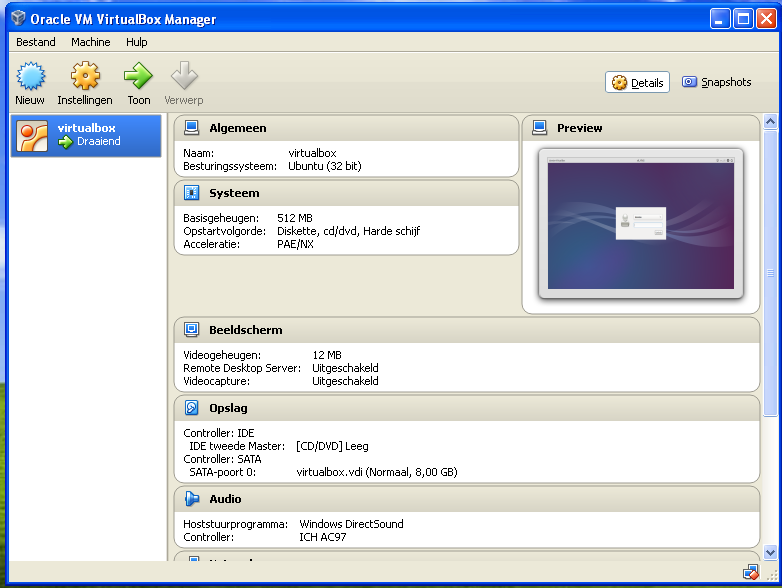
\includegraphics[width=.8\paperwidth,height=.7\paperheight,keepaspectratio]{../../pictures/virtualbox1.png}
	}
\end{frame}


\begin{frame}{Tools: The linux command line}
	a.k.a. the {\tt terminal}, {\tt shell} or, more specifically, {\tt bash}\\
	\makebox[\linewidth]{
		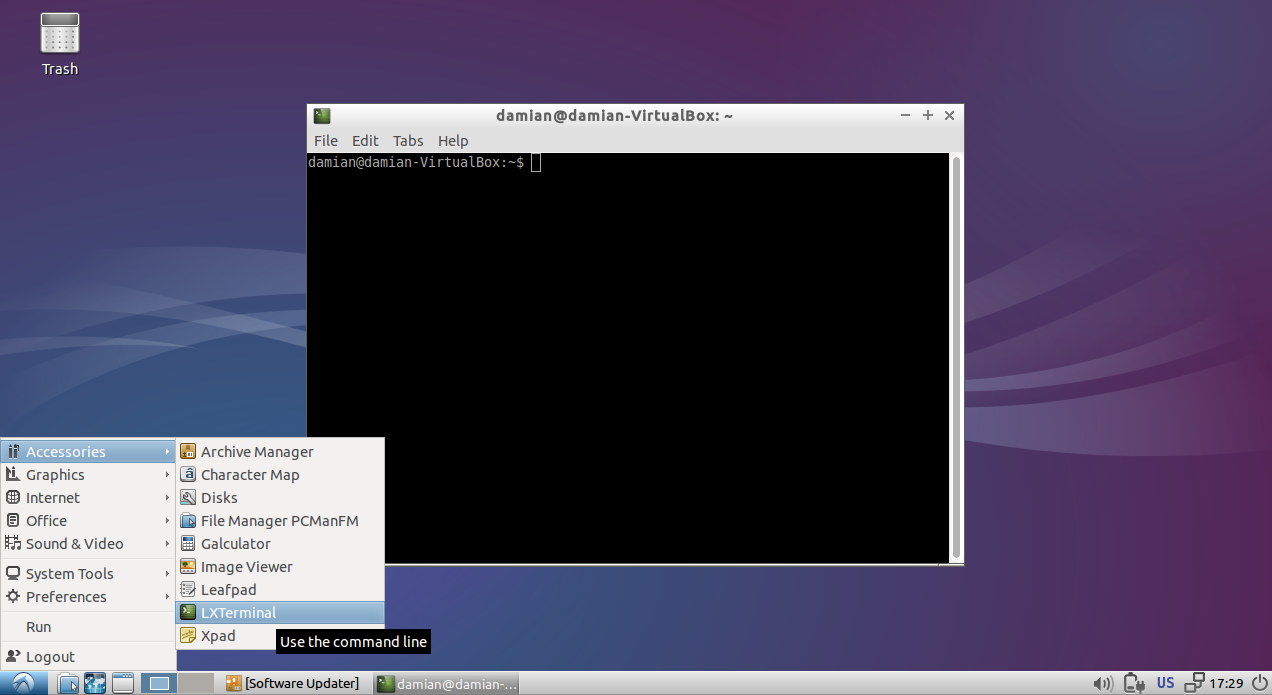
\includegraphics[width=\paperwidth,height=.8\paperheight,keepaspectratio]{../../pictures/virtualbox-bash.png}
	}
\end{frame}

\begin{frame}{Tools: The linux command line}
	%a.k.a. {\tt shell}, {\tt bash} or {\tt terminal}
	\begin{block}{Why?}<2->
		\begin{itemize}
			\item<3-> Direct access to your computer's functions
			\item<4-> In contrast to point-and-click programs, command line programs can easily be linked to each other, scripted, \ldots
			\item<5-> Suitable for handling even huge files
			\begin{itemize}
				\item<6-> You simply cannot open them in many GUI programs
				\item<6-> \ldots or it takes ages
				\item<6-> The command line allows you to do such things without problems
			\end{itemize}
			\item<7->It is reproducible (ever tried to explain to your parents on the phone where they have to click?)
		\end{itemize}
	\end{block}
\end{frame}




{\setbeamercolor{background canvas}{bg=black}
	\begin{frame}[plain]
		\color{red}\huge{There are endless tutorials, cheat sheets, videos \ldots online. Google it!}
		\makebox[\linewidth]{
			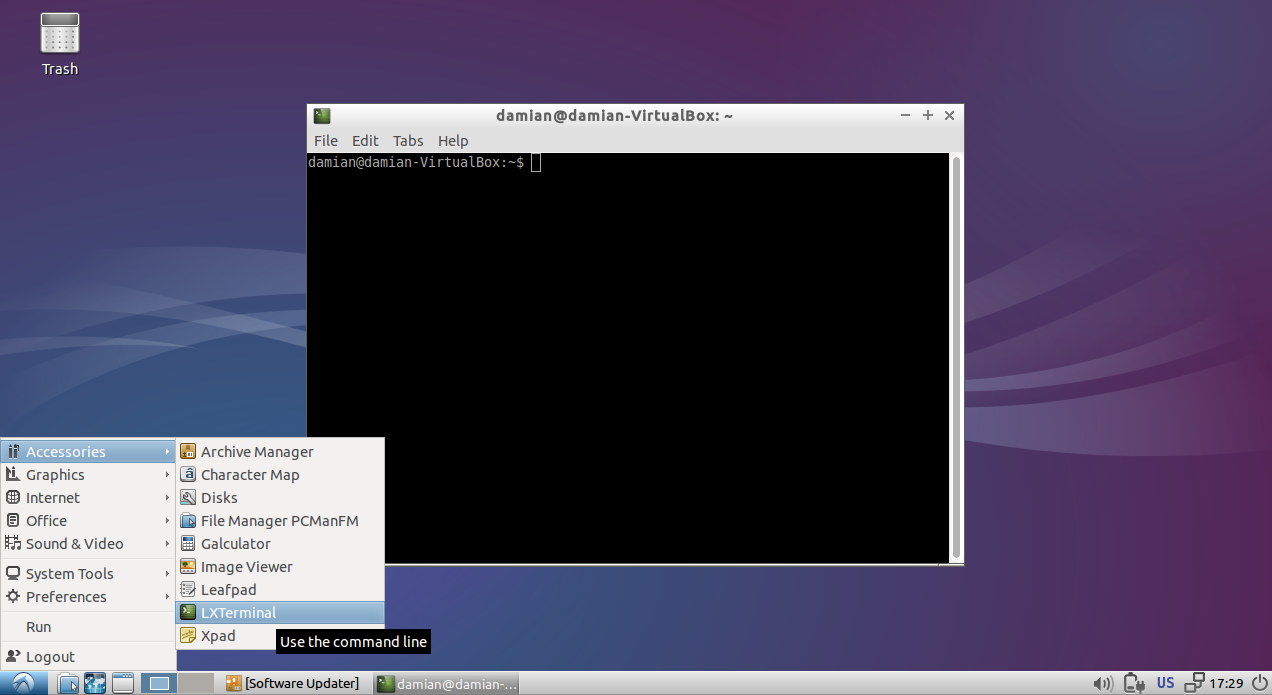
\includegraphics[width=\paperwidth,height=\paperheight,keepaspectratio]{../../pictures/virtualbox-bash.png}
		}
	\end{frame}
}


\begin{frame}
	Exercise 
	
	\vspace{1cm}
	\textbf{Take the book.\\Follow the instructions in Chapter 2.}
	
	Observe how you could do the same thing with the graphical interface.
\end{frame}




\section{Writing and running Python code}

\begin{frame}
	A language, not a program:\\
	\textbf{Python}
\end{frame}


\begin{frame}{Python}
	\begin{block}{What?}<1->
		\begin{itemize}
			\item A language, not a specific program
			\item Huge advantage: flexibility, portability
			\item One of \emph{the} languages for data analysis. \tiny{(The other one is R.)}
		\end{itemize}
	\end{block}
	
	\begin{block}{Which version?}<3->
		We use Python 3. \\ 
		\footnotesize{\url{http://www.google.com} or \url{http://www.stackexchange.com} still offer a lot of Python2-code, but that can easily be adapted. Most notable difference: In Python 2, you write {\tt print "Hi"}, this has changed to {\tt print ("Hi")}}\\
	\end{block}
\end{frame}



\begin{frame}{If it's not a program, how do you work with it?}
	\begin{block}{Interactive mode}<1->
		\begin{itemize}
			\item Just type {\tt ipython3} (if not available: {\tt python3})on the command line, and you can start entering Python commands {\tiny{(You can leave again by entering {\tt quit()})}}
			\item Great for quick try-outs, but you cannot even save your code
		\end{itemize}
	\end{block}
	
	\begin{block}{An editor of your choice}<2->
		\begin{itemize}
			\item Write your program in any text editor, save it as {\tt myprog.py}
			\item and run it from the command line with {\tt ./myprog.py} or {\tt python3 myprog.py}
		\end{itemize}
	\end{block}
\end{frame}


\begin{frame}{If it's not a program, how do you start it?}
	\begin{block}{An IDE (Integrated Development Environment)}<1->
		\begin{itemize}
			\item Provides an interface
			\item Both quick interactive try-outs and writing larger programs
			\item We use spyder, which looks a bit like RStudio (and to some extent like Stata)
		\end{itemize}
	\end{block}


\begin{block}{Jupyter Notebook}<2->
	\begin{itemize}
		\item Runs in your browser
		\item Stores results and text along with code
		\item Great for \emph{interactive} playing with data and for sharing results
	\end{itemize}
\end{block}

\end{frame}


{\setbeamercolor{background canvas}{bg=black}
	\begin{frame}[plain]
		\makebox[\linewidth]{
			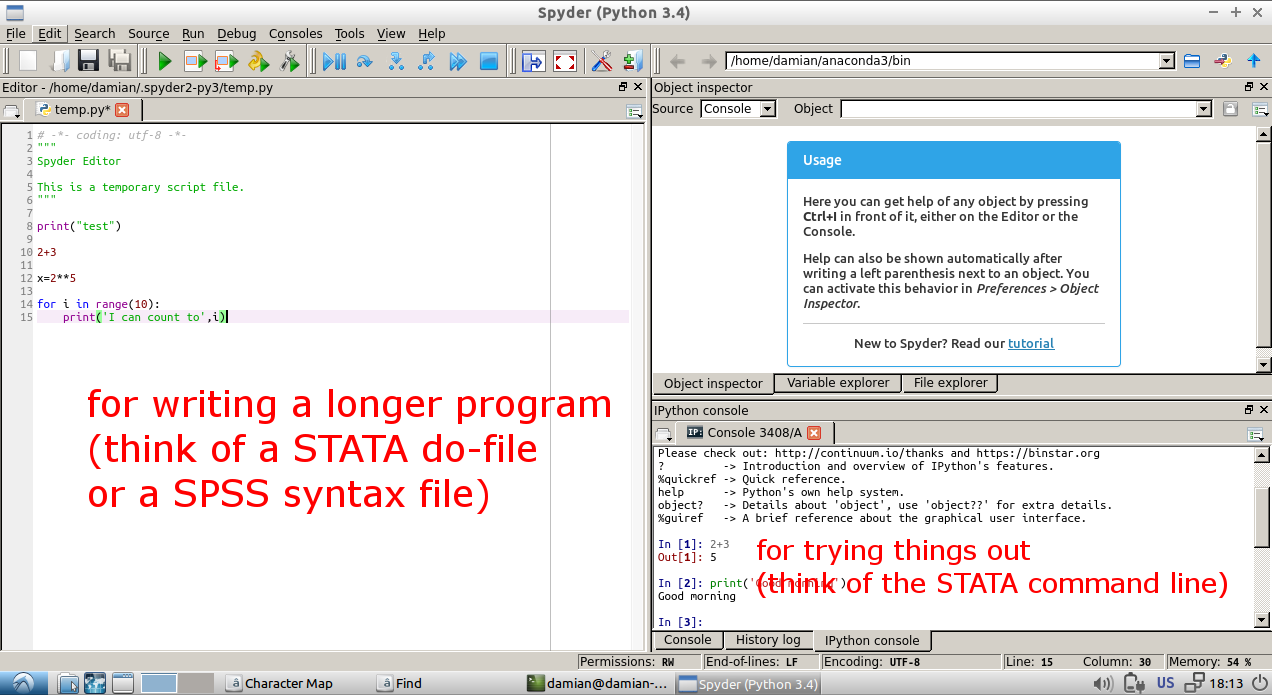
\includegraphics[width=\paperwidth,height=\paperheight,keepaspectratio]{../../pictures/spyder-uitleg.png}
		}
	\end{frame}

	\begin{frame}[plain]
		\makebox[\linewidth]{
			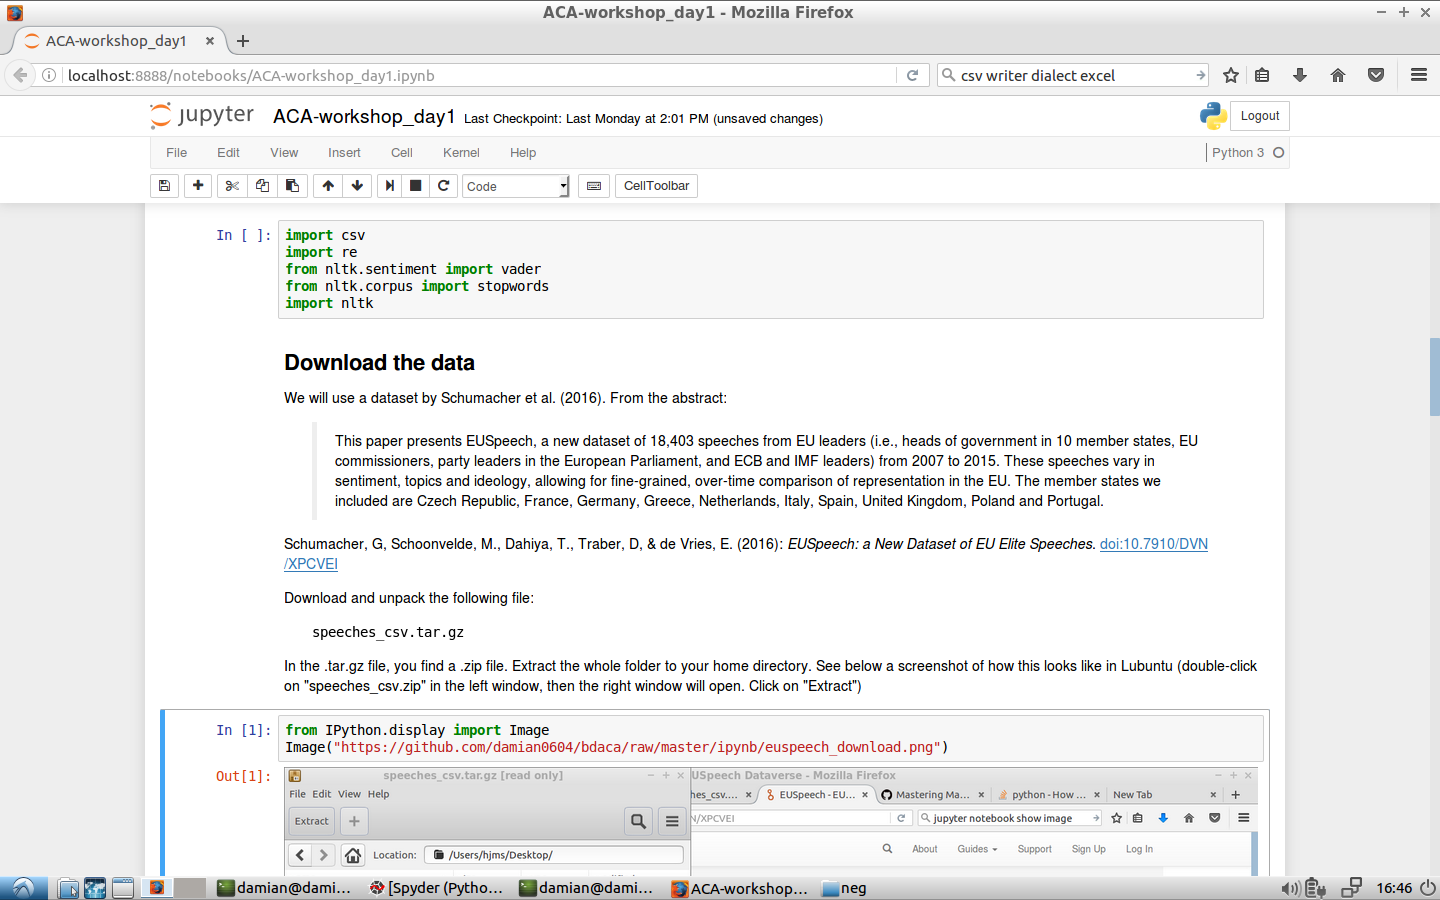
\includegraphics[width=\paperwidth,height=\paperheight,keepaspectratio]{../../pictures/jupyternotebook2.png}
		}
	\end{frame}
	
}






\begin{frame}[plain]
	Let's start up a Python environment and write a Hello-world-program!
\end{frame}


\begin{frame}[fragile]{Start playing!}
\textbf{1. Run a program that greets you.}\\
The code for this is 
\begin{lstlisting}
print("Hello world")
\end{lstlisting}
After that, do some calculations. You can do that in a similar way:
\begin{lstlisting}
a=2
print(a*3)
\end{lstlisting}
Just play around. \\ 
Repeat your exercise in different environments (command line shell, spyder, jupyter notebook).

%\vspace{.5cm}
%\textbf{Additional ressources}\\
%Codecademy course on Python
%\url{https://www.codecademy.com/learn/python}

\end{frame}



\begin{frame}[fragile]{Start playing!}

	\textbf{2. Write a program that converts centimeters to inches}\\

	Take a variable with the number of centimeters as input and print a nicely formatted answer that gives the value in inches. 1 inch = 2.54 cm.

	Printing several things in a row can be done like this:
\begin{lstlisting}
print("The answer is",42)
\end{lstlisting}	
	
	\vspace{.5cm}
	\textbf{Additional ressources}\\
	Codecademy course on Python
	\url{https://www.codecademy.com/learn/python}
	
\end{frame}



\section{Next meetings}
\begin{frame}{}
Next meetings
\end{frame}


\begin{frame}{Week 2: Getting started with Python}

\begin{block}{Monday, 12--2}
Lecture.
\\Chapter 4.
\end{block}


\begin{block}{Wednesday, 14--2}
Lab Session.
\\ Exercise A1.
\end{block}



\end{frame}




\end{document}


